\newgeometry{margin=85pt}
\chapter*{Casos prácticos}
\setcounter{chapter}{6} 
\setcounter{section}{0}
\addcontentsline{toc}{chapter}{Casos prácticos}
En este capítulo, vamos a ver los resultados obtenidos de poner en práctica algunos de los conceptos comentados a lo largo del trabajo.

\section{Centros de Atención Primaria por Municipios}

\subsection{Captura de información geográfica sobre Municipios}
Como vimos en la selección \ref{sec:fuentes}, IDENA en el mayor proveedor de datos geográficos de la Comunidad Foral de Navarra.
De toda la información que expone, hemos descargado una capa vectorial con los municipios de Navarra definida en el Catastro.
Para ello, hemos empleado dos formas distintas de descargar los datos y hemos empleado dos tecnologías distintas para cargar los datos:
\begin{itemize}
    \item Descarga de fichero Shapefile y cargar en QGIS
    
    \begin{enumerate}
        \item Acceder al cuadro de herramientas del visor web \cite{IDENA}.         
        \item Ir a la sección “capas disponibles”, en donde se muestra el catálogo de capas que expone IDENA, y seleccionar la que se llama “Municipios de Navarra (Catastro)”.
        
        \begin{figure}[H]
            \centering
            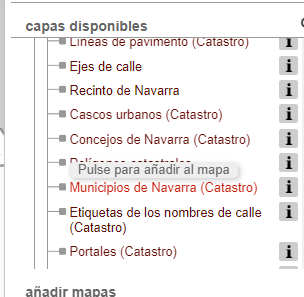
\includegraphics[width=0.30\textwidth]{Imagenes/caso-practico/capas-disponibles.png}
        \end{figure}

        \item Comprobar que la capa aparece en la sección “capas cargadas” y que se visualiza en el mapa.
        
        \begin{figure}[H]
            \centering
            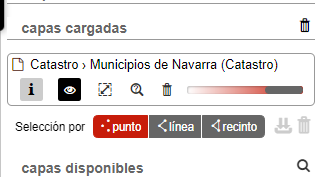
\includegraphics[width=0.30\textwidth]{Imagenes/caso-practico/capas-cargadas.png}
        \end{figure}

        \item Exportar la capa desde la sección de “descarga”. Elegimos la opción de capa vectorial y el formato Shapefile.
        
        \begin{figure}[H]
            \centering
            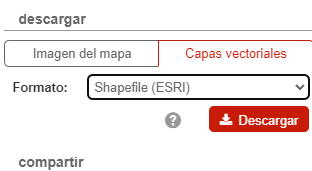
\includegraphics[width=0.30\textwidth]{Imagenes/caso-practico/descargar.png}
        \end{figure}

        \item Obtenemos un fichero comprimido que contiene todos los archivos del formato Shapefile, el cual tenemos que descomprimir.
        
        \item Importar la capa en QGIS. “Capa”; “Añadir capa”; “Añadir capa vectorial...”\\
        Una vez que tenemos cargada la capa en QGIS, podemos visualizar la tabla de atributos y seleccionar los objetos mediante ellos. 
        Como podemos ver en la siguiente tabla, cada municipio, además de su nombre, contiene información sobre su perímetro y el área que ocupa.   
        \begin{figure}[H]
            \centering
            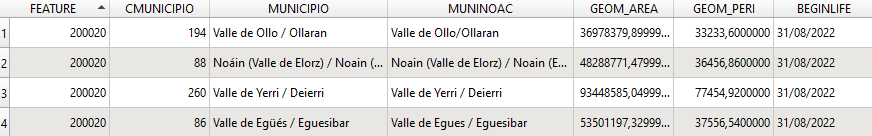
\includegraphics[width=0.90\textwidth, height=0.10\textheight]{Imagenes/caso-practico/atrubutos-municipios-qgis.png}
        \end{figure}

        \begin{figure}[H]
            \centering
            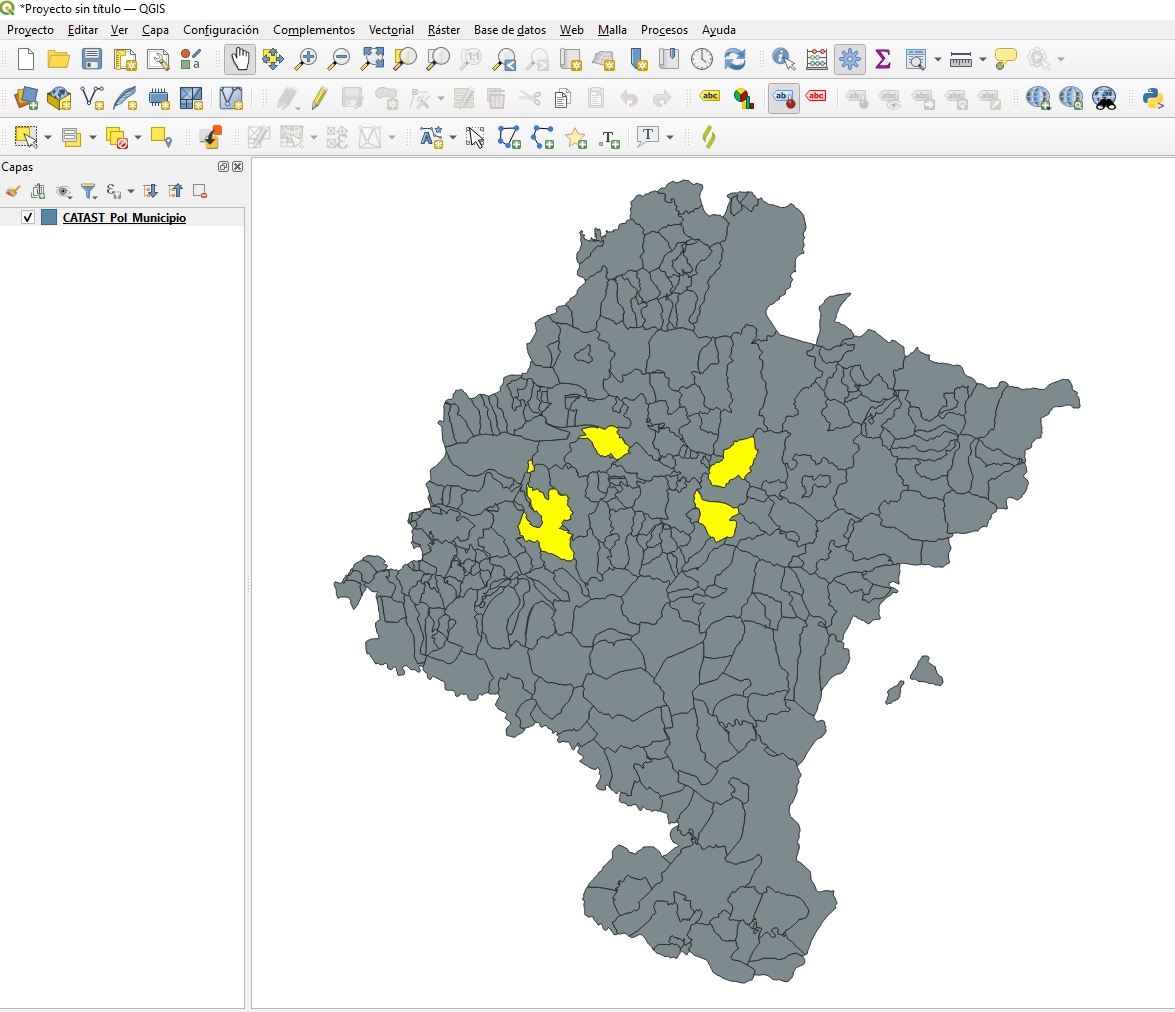
\includegraphics[width=0.85\textwidth]{Imagenes/caso-practico/municipios-qgis.png}
            \caption{Municipios Navarra visualizados en QGIS} \label{fig:municipios-qgis}
        \end{figure}
        En la figura \ref{fig:municipios-qgis}, vemos visualizados en QGIS la capa de los municipios que nos hemos descargado.
        En este caso, aparecen resaltados en color amarillo aquellos municipios cuyo nombre contiene la palabra “Valle”.
        
        Cabe destacar que la misma capa la podemos descargar en formato KML y cargarla en Google Earth. 
        Aunque la visualización resulta más amigable, Google Earth no dispone de las herramientas para el análisis espacial con las que cuenta QGIS.
    \end{enumerate}

    \newpage

    \item Petición web mediante el protocolo WFS y cargar en GeoDataFrame\\
    Para esta segunda forma, hemos empleado el lenguaje de programación Python para la manipulación de datos geográficos.
    
    \begin{enumerate}
        \item El primer paso es importar las librerías que vamos a utilizar.
        Por un lado la librería Request para realizar la petición al servicio WFS de IDENA y por otro lado la librería GeoPandas.
        Esta última es una ampliación de la biblioteca Pandas, empleada en ciencia de datos, a la que le agrega un soporte para el manejo de datos geoespaciales.

\begin{tcolorbox}[breakable, size=fbox, boxrule=1pt, colback=cellbackground, colframe=cellborder, fontupper=\footnotesize]
    \prompt{In}{incolor}{1}{\boxspacing}
    \begin{Verbatim}[commandchars=\\\{\}]
    \PY{k+kn}{import} \PY{n+nn}{requests}
    \PY{k+kn}{import} \PY{n+nn}{geopandas} \PY{k}{as} \PY{n+nn}{gpd}
    \end{Verbatim}
\end{tcolorbox}

        \item Realizamos la petición de los municipios de Navarra al servicio WFS de IDENA y recogemos la respuesta en formato JSON.

\begin{tcolorbox}[breakable, size=fbox, boxrule=1pt, colback=cellbackground, colframe=cellborder, fontupper=\footnotesize]
    \prompt{In}{incolor}{2}{\boxspacing}
    \begin{Verbatim}[commandchars=\\\{\}]
    \PY{n}{url} \PY{o}{=} \PY{l+s+s2}{\PYZdq{}\PYZdq{}\PYZdq{}}\PY{l+s+s2}{https://idena.navarra.es/ogc/wfs}\PY{l+s+s2}{\PYZdq{}\PYZdq{}\PYZdq{}}
    \PY{n}{parameters} \PY{o}{=} \PY{p}{\PYZob{}}
    \PY{l+s+s1}{\PYZsq{}}\PY{l+s+s1}{service}\PY{l+s+s1}{\PYZsq{}}\PY{p}{:} \PY{l+s+s1}{\PYZsq{}}\PY{l+s+s1}{WFS}\PY{l+s+s1}{\PYZsq{}}\PY{p}{,}
    \PY{l+s+s1}{\PYZsq{}}\PY{l+s+s1}{version}\PY{l+s+s1}{\PYZsq{}}\PY{p}{:} \PY{l+s+s1}{\PYZsq{}}\PY{l+s+s1}{2.0.0}\PY{l+s+s1}{\PYZsq{}}\PY{p}{,}
    \PY{l+s+s1}{\PYZsq{}}\PY{l+s+s1}{typename}\PY{l+s+s1}{\PYZsq{}}\PY{p}{:} \PY{l+s+s1}{\PYZsq{}}\PY{l+s+s1}{IDENA:CATAST\PYZus{}Pol\PYZus{}Municipio}\PY{l+s+s1}{\PYZsq{}}\PY{p}{,}
    \PY{l+s+s1}{\PYZsq{}}\PY{l+s+s1}{srsname}\PY{l+s+s1}{\PYZsq{}}\PY{p}{:} \PY{l+s+s1}{\PYZsq{}}\PY{l+s+s1}{EPSG:4326}\PY{l+s+s1}{\PYZsq{}}\PY{p}{,}
    \PY{l+s+s1}{\PYZsq{}}\PY{l+s+s1}{request}\PY{l+s+s1}{\PYZsq{}}\PY{p}{:} \PY{l+s+s1}{\PYZsq{}}\PY{l+s+s1}{getFeature}\PY{l+s+s1}{\PYZsq{}}\PY{p}{,}
    \PY{l+s+s1}{\PYZsq{}}\PY{l+s+s1}{outputFormat}\PY{l+s+s1}{\PYZsq{}}\PY{p}{:} \PY{l+s+s1}{\PYZsq{}}\PY{l+s+s1}{json}\PY{l+s+s1}{\PYZsq{}}
    \PY{p}{\PYZcb{}}
    \PY{n}{response} \PY{o}{=} \PY{n}{requests}\PY{o}{.}\PY{n}{post}\PY{p}{(}\PY{n}{url}\PY{p}{,} \PY{n}{data}\PY{o}{=}\PY{n}{parameters}\PY{p}{)}
    \PY{n}{json} \PY{o}{=} \PY{n}{response}\PY{o}{.}\PY{n}{json}\PY{p}{(}\PY{p}{)}
    \end{Verbatim}
\end{tcolorbox}

        \item Construimos un GeoDataFrame a partir del JSON obtenido. Los GeoDataFrame son estructura en forma de tabla en la que cada fila corresponde a un objeto GeoSeries.
        Los GeoSeries son vectores que guardan tanto las propiedades geométricas como los atributos de objetos. En nuestro caso, guarda la geometría de cada municipio, 
        junto a los atributos que hemos visto anteriormente (nombre, perímetro, área, etc.).
\begin{tcolorbox}[breakable, size=fbox, boxrule=1pt, colback=cellbackground, colframe=cellborder, fontupper=\footnotesize]
    \prompt{In}{incolor}{3}{\boxspacing}
    \begin{Verbatim}[commandchars=\\\{\}]
    \PY{n}{municipiosGDF} \PY{o}{=} \PY{n}{gpd}\PY{o}{.}\PY{n}{GeoDataFrame}\PY{o}{.}\PY{n}{from\PYZus{}features}\PY{p}{(}\PY{n}{json}\PY{p}{[}\PY{l+s+s2}{\PYZdq{}}\PY{l+s+s2}{features}\PY{l+s+s2}{\PYZdq{}}\PY{p}{]}\PY{p}{)}
    \end{Verbatim}
\end{tcolorbox}
\begin{tcolorbox}[breakable, size=fbox, boxrule=.5pt, pad at break*=1mm, opacityfill=0, fontupper=\tiny]
    \prompt{Out}{outcolor}{3}{\boxspacing}
    \begin{Verbatim}[commandchars=\\\{\}]
                                                    geometry  FEATURE  CMUNICIPIO  MUNICIPIO  \textbackslash{}
    190  MULTIPOLYGON (((-1.84177 42.84037, -1.84189 42{\ldots}   200020         194    Valle de Ollo / Ollaran
    282  MULTIPOLYGON (((-1.63079 42.77244, -1.63063 42{\ldots}   200020          88    Noáin (Valle de Elorz) / Noain (Elortzibar)
    297  MULTIPOLYGON (((-2.03778 42.80587, -2.03807 42{\ldots}   200020         260    Valle de Yerri / Deierri
    337  MULTIPOLYGON (((-1.57393 42.83506, -1.57391 42{\ldots}   200020          86    Valle de Egüés / Eguesibar                
    
                                            MUNINOAC    GEOM\_AREA  GEOM\_PERI  BEGINLIFE
    190                        Valle de Ollo/Ollaran  36978379.90   33233.60    01/09/2022
    282  Noain (Valle de Elorz) / Noain (Elortzibar)  48288771.48   36456.86    01/09/2022
    297                     Valle de Yerri / Deierri  93448585.05   77454.92    01/09/2022
    337                   Valle de Egues / Eguesibar  53501197.33   37556.54    01/09/2022
    \end{Verbatim}
\end{tcolorbox}

        \item Visualizamos los municipios.
\begin{tcolorbox}[breakable, size=fbox, boxrule=1pt, colback=cellbackground, colframe=cellborder, fontupper=\footnotesize]
    \prompt{In}{incolor}{4}{\boxspacing}
    \begin{Verbatim}[commandchars=\\\{\}]
    \PY{n}{municipiosGDF}\PY{o}{.}\PY{n}{plot}\PY{p}{(}\PY{p}{)}
    \end{Verbatim}
\end{tcolorbox}
        \begin{center}
            \adjustimage{max size={0.75\linewidth}{0.75\paperheight}}{Imagenes/caso-practico/plot-municipios.png}
        \end{center}
    \end{enumerate} 
\end{itemize}

\subsection{Añadir capas de Centros de Atención Primaria}
El primer paso es la descarga de la capa vectorial, correspondiente a las localizaciones de los centros de atención primaria de Navarra.
Para ello, hacemos la petición al servicio WFS de IDENA desde código Python, al igual que con los municipios.

\begin{tcolorbox}[breakable, size=fbox, boxrule=1pt, pad at break*=1mm,colback=cellbackground, colframe=cellborder, fontupper=\footnotesize]
    \prompt{In}{incolor}{5}{\boxspacing}
    \begin{Verbatim}[commandchars=\\\{\}]
    \PY{n}{url} \PY{o}{=} \PY{l+s+s2}{\PYZdq{}\PYZdq{}\PYZdq{}}\PY{l+s+s2}{https://idena.navarra.es/ogc/wfs}\PY{l+s+s2}{\PYZdq{}\PYZdq{}\PYZdq{}}
    \PY{n}{parameters} \PY{o}{=} \PY{p}{\PYZob{}}
    \PY{l+s+s1}{\PYZsq{}}\PY{l+s+s1}{service}\PY{l+s+s1}{\PYZsq{}}\PY{p}{:} \PY{l+s+s1}{\PYZsq{}}\PY{l+s+s1}{WFS}\PY{l+s+s1}{\PYZsq{}}\PY{p}{,}
    \PY{l+s+s1}{\PYZsq{}}\PY{l+s+s1}{version}\PY{l+s+s1}{\PYZsq{}}\PY{p}{:} \PY{l+s+s1}{\PYZsq{}}\PY{l+s+s1}{2.0.0}\PY{l+s+s1}{\PYZsq{}}\PY{p}{,}
    \PY{l+s+s1}{\PYZsq{}}\PY{l+s+s1}{typename}\PY{l+s+s1}{\PYZsq{}}\PY{p}{:} \PY{l+s+s1}{\PYZsq{}}\PY{l+s+s1}{IDENA:DOTACI\PYZus{}Sym\PYZus{}SNSPrimaria}\PY{l+s+s1}{\PYZsq{}}\PY{p}{,}
    \PY{l+s+s1}{\PYZsq{}}\PY{l+s+s1}{srsname}\PY{l+s+s1}{\PYZsq{}}\PY{p}{:} \PY{l+s+s1}{\PYZsq{}}\PY{l+s+s1}{EPSG:4326}\PY{l+s+s1}{\PYZsq{}}\PY{p}{,}
    \PY{l+s+s1}{\PYZsq{}}\PY{l+s+s1}{request}\PY{l+s+s1}{\PYZsq{}}\PY{p}{:} \PY{l+s+s1}{\PYZsq{}}\PY{l+s+s1}{getFeature}\PY{l+s+s1}{\PYZsq{}}\PY{p}{,}
    \PY{l+s+s1}{\PYZsq{}}\PY{l+s+s1}{outputFormat}\PY{l+s+s1}{\PYZsq{}}\PY{p}{:} \PY{l+s+s1}{\PYZsq{}}\PY{l+s+s1}{json}\PY{l+s+s1}{\PYZsq{}}
    \PY{p}{\PYZcb{}}
    \PY{n}{response} \PY{o}{=} \PY{n}{requests}\PY{o}{.}\PY{n}{post}\PY{p}{(}\PY{n}{url}\PY{p}{,} \PY{n}{data}\PY{o}{=}\PY{n}{parameters}\PY{p}{)}
    \PY{n}{json} \PY{o}{=} \PY{n}{response}\PY{o}{.}\PY{n}{json}\PY{p}{(}\PY{p}{)}
    \PY{n}{centrosAtencionPrimariaGDF} \PY{o}{=} \PY{n}{gpd}\PY{o}{.}\PY{n}{GeoDataFrame}\PY{o}{.}\PY{n}{from\PYZus{}features}\PY{p}{(}\PY{n}{json}\PY{p}{[}\PY{l+s+s2}{\PYZdq{}}\PY{l+s+s2}{features}\PY{l+s+s2}{\PYZdq{}}\PY{p}{]}\PY{p}{)}
    \PY{n}{centrosAtencionPrimariaGDF}\PY{o}{.}\PY{n}{head}\PY{p}{(}\PY{p}{)}
    \end{Verbatim}
\end{tcolorbox}
    
Mostramos algunos ejemplos de centros de salud. Vemos que estos presentan una geometría en forma de Punto (POINT), al contrario que los municipios,
que podían estar formados por uno o varios polígonos (MULTIPOLYGON).

\begin{tcolorbox}[breakable, size=fbox, boxrule=.5pt, pad at break*=1mm, opacityfill=0, fontupper=\tiny]
    \prompt{Out}{outcolor}{5}{\boxspacing}
    \begin{Verbatim}[commandchars=\\\{\}]
                        geometry  FEATURE IDCENSAN  CENSAN                          CZONA   ZONA            CENTSINGDP
    0  POINT (-1.60207 42.05893)  7400025    00001  Centro de Salud de Tudela Este  46      TUDELA ESTE     802
    1  POINT (-1.61057 42.06222)  7400025    00002  Centro de Salud de Tudela Oeste 45      TUDELA OESTE    802
    2  POINT (-1.68023 42.00230)  7400025    00003  Centro de Salud de Cascante     50      CASCANTE        238
    3  POINT (-1.44259 41.97833)  7400025    00004  Centro de Salud de Buñuel       51      BUÑUEL          223
    4  POINT (-1.80554 42.08284)  7400025    00005  Centro de Salud de Cintruénigo  49      CINTRUÉNIGO     244
    
         POBLACION              DIRECCION CODPOSTAL      X25830      Y25830  BEGINLIFE
    0       TUDELA  JUAN A. FERNANDEZ, 12     31500  615667.221  4657264.89  17/06/2019
    1       TUDELA            GAYARRE, 17     31500  614958.282  4657617.90  17/06/2019
    2     CASCANTE     AVDA. CARIDAD, S/N     31520  609297.095  4650873.88  17/06/2019
    3       BUÑUEL    CRISTOBAL COLON, 19     31540  629026.275  4648543.31  17/06/2019
    4  CINTRUENIGO              RIBERA, 2     31592  598794.444  4659663.89  17/06/2019
\end{Verbatim}
\end{tcolorbox}

Generamos un campo nuevo que indique si el municipio cuneta con algún centro de atención primaria.

\begin{tcolorbox}[breakable, size=fbox, boxrule=1pt, pad at break*=1mm,colback=cellbackground, colframe=cellborder, fontupper=\footnotesize]
    \prompt{In}{incolor}{6}{\boxspacing}
    \begin{Verbatim}[commandchars=\\\{\}]
    \PY{n}{municipiosGDF}\PY{p}{[}\PY{l+s+s1}{\PYZsq{}}\PY{l+s+s1}{TieneCentro}\PY{l+s+s1}{\PYZsq{}}\PY{p}{]} \PY{o}{=} \PY{p}{[}\PY{n}{centrosAtencionPrimariaGDF}\PY{o}{.}\PY{n}{within}\PY{p}{(}\PY{n}{geo}\PY{p}{)}\PY{o}{.}\PY{n}{any}\PY{p}{(}\PY{p}{)} \PY{k}{for} \PY{n}{key}\PY{p}{,} \PY{n}{geo} \PY{o+ow}{in} \PY{n}{municipiosGDF}\PY{o}{.}\PY{n}{geometry}\PY{o}{.}\PY{n}{items}\PY{p}{(}\PY{p}{)}\PY{p}{]}
    \end{Verbatim}
\end{tcolorbox}        

\subsection{Resultado final}

\begin{figure}[H]
    \centering
    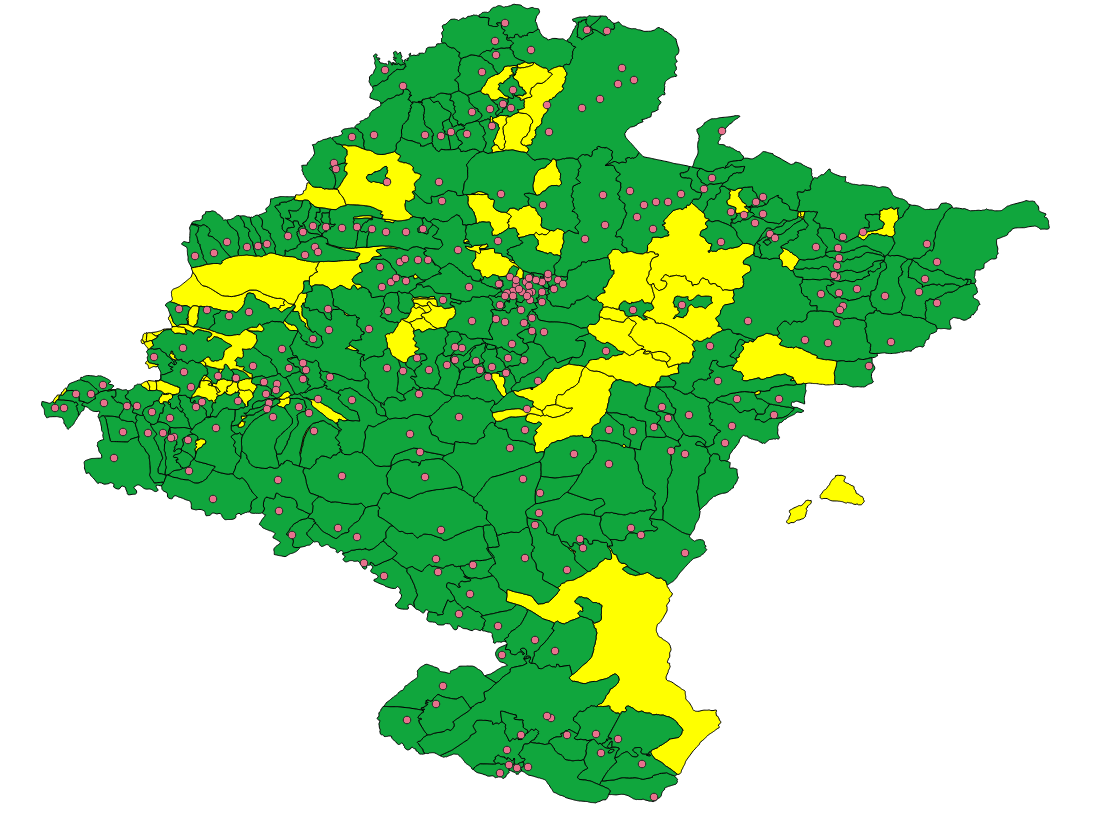
\includegraphics[width=0.84\textwidth]{Imagenes/caso-practico/municipios-sin-centro.png}
    \caption{Municipios sin Centro de Atención Primaria} \label{fig:municipios-sin-centro}
\end{figure}
La figura \ref{fig:municipios-sin-centro} muestra sobre el mapa de Navarra los puntos en el que se localizan todos los centro de atención primaria.
Los municipios que no tinen ninguno aparecen en color amarillo, mientras que los municipios que tiene al menos un centro de atención primaria aparecen en color verde.

Podemos obtener los 10 municipios con mayor extensión, es decir, mayor área, que carecen de centro de atención primaria.

\begin{tcolorbox}[breakable, size=fbox, boxrule=.5pt, pad at break*=1mm, opacityfill=0, fontupper=\tiny]
    \prompt{Out}{outcolor}{ }{\boxspacing}
    \begin{Verbatim}[commandchars=\\\{\}]
                                             MUNICIPIO  GEOM\_AREA      TieneCentro
    172                                Bardenas Reales  4.184495e+08    False
    152                                   Arce / Artzi  1.463562e+08    False
    188                               Sierra de Urbasa  1.144517e+08    False
    287                                        Larraun  1.077661e+08    False
    195                                   Leoz / Leotz  9.622492e+07    False
    137                      Romanzado / Erromantzatua  9.169286e+07    False
    291                             Lónguida / Longida  9.071720e+07    False
    294  Lizoain-Arriasgoiti / Lizoainibar-Arriasgoiti  6.523998e+07    False
    295                                     Izagaondoa  5.960535e+07    False
    238                                      Ibargoiti  5.405204e+07    False
    \end{Verbatim}
\end{tcolorbox}

\section{Río Ebro}

\subsection{Captura y procesado de información sobre ríos}
Al igual que en el caso anterior, lo primero es importar las librerías que vamos a utilizar.
\begin{tcolorbox}[breakable, size=fbox, boxrule=1pt, pad at break*=1mm,colback=cellbackground, colframe=cellborder, fontupper=\footnotesize]
    \prompt{In}{incolor}{1}{\boxspacing}
    \begin{Verbatim}[commandchars=\\\{\}]
    \PY{k+kn}{import} \PY{n+nn}{requests}
    \PY{k+kn}{import} \PY{n+nn}{geopandas} \PY{k}{as} \PY{n+nn}{gpd}
    \PY{k+kn}{import} \PY{n+nn}{numpy} \PY{k}{as} \PY{n+nn}{np}
    \PY{k+kn}{from} \PY{n+nn}{shapely}\PY{n+nn}{.}\PY{n+nn}{geometry} \PY{k+kn}{import} \PY{n}{box, Polygon}
    \PY{k+kn}{from} \PY{n+nn}{PIL} \PY{k+kn}{import} \PY{n}{Image}\PY{p}{,} \PY{n}{ImageDraw}
    \PY{k+kn}{import} \PY{n+nn}{matplotlib}\PY{n+nn}{.}\PY{n+nn}{pyplot} \PY{k}{as} \PY{n+nn}{plt}
    \PY{k+kn}{import} \PY{n+nn}{random}
    \PY{k+kn}{import} \PY{n+nn}{io}
    \end{Verbatim}
\end{tcolorbox}

\begin{figure}[H]
    \centering
    \subfigure[Capa original]{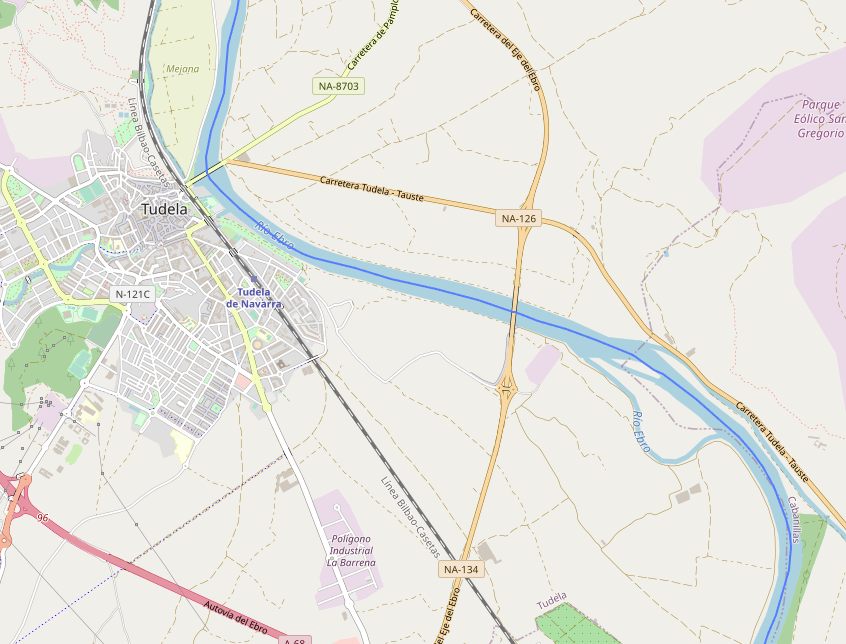
\includegraphics[width=0.35\columnwidth]{Imagenes/caso-practico/rio-ebro-tudela.png}}
    \subfigure[Zona buffer]{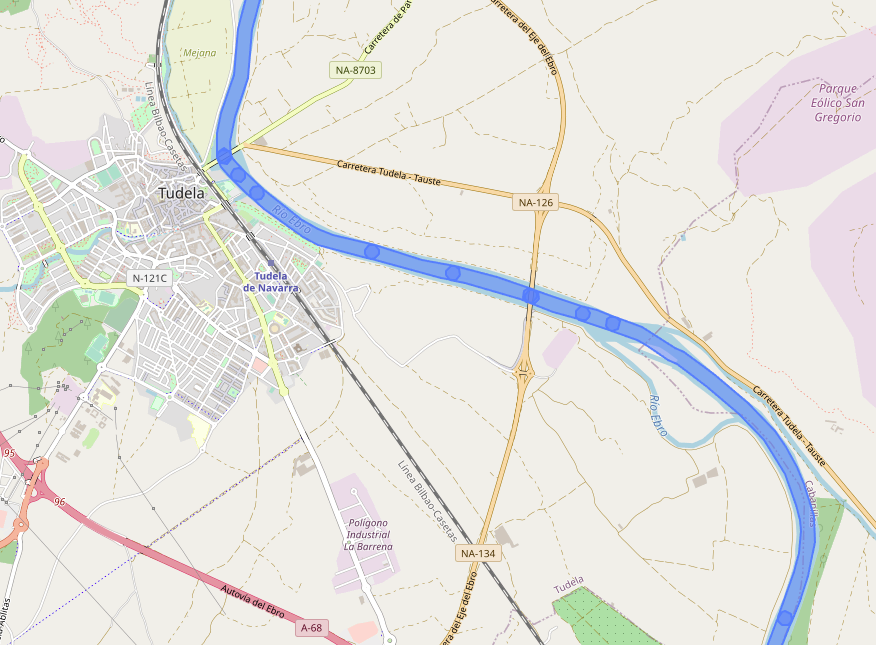
\includegraphics[width=0.35\columnwidth]{Imagenes/caso-practico/rio-ebro-tudela2.png}}
    \subfigure[Unión de polígonos]{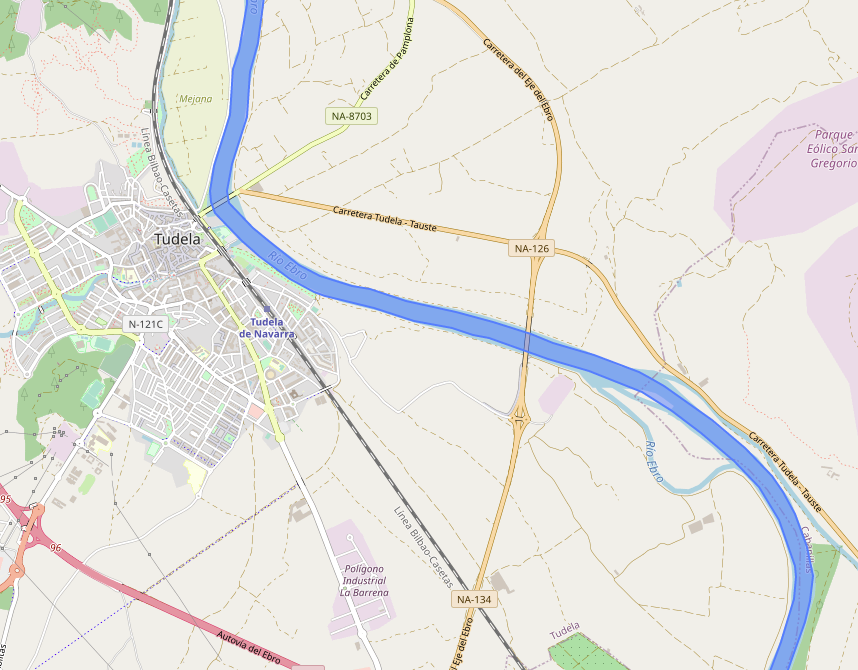
\includegraphics[width=0.35\columnwidth]{Imagenes/caso-practico/rio-ebro-tudela3.png}}
    \caption{Selección del río Ebro a su paso por Tudela} \label{fig:ebro-tudela} 
\end{figure} 
En esta primera parte hemos cargado la capa de las corrientes principales de Navarra y hemos generado otra con el cauce del río Ebro.
Los pasos intermedios se observan en la figura \ref{fig:ebro-tudela} sobre el río Ebro a su paso por Tudela.
\begin{itemize}
    \item El punto \textit{a} muestra la capa original de IDENA (punto 1.2), que consta de una línea situada en la mitad del cauce del río.
    \item El punto \textit{b} muestra la zona buffer generada  (punto 1.3), en la que se ha aumentado el ancho de la la línea de la capa original,
    Lo que permite apreciar que la capa original no estaba formada por una sola línea. 
    \item El punto \textit{c} muestra la unión de todas las zonas buffer generadas (punto 1.4)
\end{itemize}

\begin{tcolorbox}[breakable, size=fbox, boxrule=1pt, pad at break*=1mm,colback=cellbackground, colframe=cellborder, fontupper=\footnotesize]
    \prompt{In}{incolor}{ }{\boxspacing}
    \begin{Verbatim}[commandchars=\\\{\}]
    \PY{c+c1}{\PYZsh{} 1.1 Leemos el fichero con la capa de las corrientes naturales de Navarra}
    \PY{n}{riosGDF} \PY{o}{=} \PY{n}{gpd}\PY{o}{.}\PY{n}{read\PYZus{}file}\PY{p}{(}\PY{l+s+s1}{\PYZsq{}}\PY{l+s+s1}{files/input/HIDROG\PYZus{}Lin\PYZus{}CorrienteNatural.shp}\PY{l+s+s1}{\PYZsq{}}\PY{p}{)} 
    \PY{c+c1}{\PYZsh{} 1.2 Seleccionamos las líneas correspondientes al río Ebro}
    \PY{n}{rioEbroGDF} \PY{o}{=} \PY{n}{riosGDF}\PY{o}{.}\PY{n}{loc}\PY{p}{[}\PY{n}{riosGDF}\PY{o}{.}\PY{n}{NOMBRE} \PY{o}{==} \PY{l+s+s2}{\PYZdq{}}\PY{l+s+s2}{Río Ebro}\PY{l+s+s2}{\PYZdq{}}\PY{p}{]}
    \PY{c+c1}{\PYZsh{} 1.3 Generamos una zona buffer de 60 metros de radio.}
    \PY{n}{rioEbroGDF\PYZus{}buffer} \PY{o}{=} \PY{n}{rioEbroGDF}\PY{o}{.}\PY{n}{buffer}\PY{p}{(}\PY{l+m+mf}{60.0}\PY{p}{)}
    \PY{n}{rioEbroGDF}\PY{o}{.}\PY{n}{geometry} \PY{o}{=} \PY{n}{rioEbroGDF\PYZus{}buffer}
    \PY{c+c1}{\PYZsh{} 1.4 Unimos todas las zonas buffer generadas}
    \PY{n}{rioEbroGDF} \PY{o}{=} \PY{n}{rioEbroGDF}\PY{o}{.}\PY{n}{dissolve}\PY{p}{(}\PY{n}{by}\PY{o}{=}\PY{l+s+s1}{\PYZsq{}}\PY{l+s+s1}{NOMBRE}\PY{l+s+s1}{\PYZsq{}}\PY{p}{)}
    \PY{c+c1}{\PYZsh{} 1.5 Modificamos el sistema de referencia}
    \PY{n}{rioEbroGDF} \PY{o}{=} \PY{n}{rioEbroGDF}\PY{o}{.}\PY{n}{to\PYZus{}crs}\PY{p}{(}\PY{n}{epsg}\PY{o}{=}\PY{l+m+mi}{4326}\PY{p}{)}
    \PY{c+c1}{\PYZsh{} 1.6 Obtenemos las coordenadas de los polígonos que forman el río Ebro}
    \PY{n}{ebro\PYZus{}points} \PY{o}{=} \PY{n}{np}\PY{o}{.}\PY{n}{array}\PY{p}{(}\PY{p}{[}\PY{n}{polygon}\PY{o}{.}\PY{n}{exterior}\PY{o}{.}\PY{n}{coords}\PY{p}{[}\PY{p}{:}\PY{o}{\PYZhy{}}\PY{l+m+mi}{1}\PY{p}{]} \PY{k}{for} \PY{n}{multipolygon} \PY{o+ow}{in} \PY{n}{rioEbroGDF}\PY{o}{.}\PY{n}{geometry} \PY{k}{for} \PY{n}{polygon} \PY{o+ow}{in} \PY{n}{multipolygon}\PY{p}{]}\PY{p}{)}
    \PY{n}{ebro\PYZus{}points} \PY{o}{=} \PY{n}{np}\PY{o}{.}\PY{n}{concatenate}\PY{p}{(}\PY{n}{ebro\PYZus{}points}\PY{p}{)}
    \end{Verbatim}
\end{tcolorbox}
\newpage
\subsection{Descarga de imágenes aéreas}
En esta segunda parte, vamos a descargar imágenes aéreas del servicio WMS de IDENA para que nos sirva como mapa de fondo.
En concreto, vamos a emplear el mapa base con ortofoto de máxima actualidad (año 2021). 
Las ortofotografías con imágenes obtenidas a partir de un vuelo digital, en este caso a una altura comprendida entre los 5200 y 7200 metros. 

Definimos los parámetros de la petición del mapa, entre los cuales pasamos un bounding box (BBOX) que limita la descarga a la zona de terreno que envuelve.
\begin{tcolorbox}[breakable, size=fbox, boxrule=1pt, pad at break*=1mm,colback=cellbackground, colframe=cellborder, fontupper=\footnotesize]
    \prompt{In}{incolor}{139}{\boxspacing}
    \begin{Verbatim}[commandchars=\\\{\}]
    \PY{n}{url} \PY{o}{=} \PY{l+s+s2}{\PYZdq{}\PYZdq{}\PYZdq{}}\PY{l+s+s2}{https://idena.navarra.es/ogc/wms}\PY{l+s+s2}{\PYZdq{}\PYZdq{}\PYZdq{}}
    \PY{n}{parameters} \PY{o}{=} \PY{p}{\PYZob{}}
        \PY{l+s+s1}{\PYZsq{}}\PY{l+s+s1}{service}\PY{l+s+s1}{\PYZsq{}}\PY{p}{:} \PY{l+s+s1}{\PYZsq{}}\PY{l+s+s1}{WMS}\PY{l+s+s1}{\PYZsq{}}\PY{p}{,}
        \PY{l+s+s1}{\PYZsq{}}\PY{l+s+s1}{version}\PY{l+s+s1}{\PYZsq{}}\PY{p}{:} \PY{l+s+s1}{\PYZsq{}}\PY{l+s+s1}{2.0.0}\PY{l+s+s1}{\PYZsq{}}\PY{p}{,}
        \PY{l+s+s1}{\PYZsq{}}\PY{l+s+s1}{LAYERS}\PY{l+s+s1}{\PYZsq{}}\PY{p}{:} \PY{l+s+s1}{\PYZsq{}}\PY{l+s+s1}{IDENA:ortofoto\PYZus{}maxima\PYZus{}actualidad}\PY{l+s+s1}{\PYZsq{}}\PY{p}{,}
        \PY{l+s+s1}{\PYZsq{}}\PY{l+s+s1}{CRS}\PY{l+s+s1}{\PYZsq{}}\PY{p}{:} \PY{l+s+s1}{\PYZsq{}}\PY{l+s+s1}{EPSG:4326}\PY{l+s+s1}{\PYZsq{}}\PY{p}{,}
        \PY{l+s+s1}{\PYZsq{}}\PY{l+s+s1}{request}\PY{l+s+s1}{\PYZsq{}}\PY{p}{:} \PY{l+s+s1}{\PYZsq{}}\PY{l+s+s1}{getMap}\PY{l+s+s1}{\PYZsq{}}\PY{p}{,}
        \PY{l+s+s1}{\PYZsq{}}\PY{l+s+s1}{format}\PY{l+s+s1}{\PYZsq{}}\PY{p}{:} \PY{l+s+s1}{\PYZsq{}}\PY{l+s+s1}{image/png}\PY{l+s+s1}{\PYZsq{}}\PY{p}{,}
        \PY{l+s+s1}{\PYZsq{}}\PY{l+s+s1}{BBOX}\PY{l+s+s1}{\PYZsq{}}\PY{p}{:} \PY{l+s+s1}{\PYZsq{}}\PY{l+s+s1}{\PYZob{}}\PY{l+s+s1}{lon\PYZus{}min,lat\PYZus{}min,lon\PYZus{}max,lat\PYZus{}max\PYZcb{}}\PY{l+s+s1}{\PYZsq{}}\PY{p}{,}
        \PY{l+s+s1}{\PYZsq{}}\PY{l+s+s1}{WIDTH}\PY{l+s+s1}{\PYZsq{}}\PY{p}{:} \PY{l+s+s1}{\PYZsq{}}\PY{l+s+s1}{256}\PY{l+s+s1}{\PYZsq{}}\PY{p}{,}
        \PY{l+s+s1}{\PYZsq{}}\PY{l+s+s1}{HEIGHT}\PY{l+s+s1}{\PYZsq{}}\PY{p}{:} \PY{l+s+s1}{\PYZsq{}}\PY{l+s+s1}{256}\PY{l+s+s1}{\PYZsq{}}
    \PY{p}{\PYZcb{}}
    \end{Verbatim}
\end{tcolorbox}

También hemos definido un par de funciones que usaremos en el solapamiento del mapa base con la capa del río Ebro.

\begin{tcolorbox}[breakable, size=fbox, boxrule=1pt, pad at break*=1mm,colback=cellbackground, colframe=cellborder, fontupper=\footnotesize]
    \prompt{In}{incolor}{159}{\boxspacing}
    \begin{Verbatim}[commandchars=\\\{\}]
    \PY{c+c1}{\PYZsh{} Obtiene un bounding box a partir del punto central y un margen a este}
    \PY{k}{def} \PY{n+nf}{get\PYZus{}bbox\PYZus{}coord}\PY{p}{(}\PY{n}{point}\PY{p}{,} \PY{n}{grow}\PY{p}{)}\PY{p}{:}
        \PY{n}{lon\PYZus{}min} \PY{o}{=} \PY{n}{point}\PY{p}{[}\PY{l+m+mi}{0}\PY{p}{]} \PY{o}{\PYZhy{}} \PY{n}{grow}
        \PY{n}{lat\PYZus{}min} \PY{o}{=} \PY{n}{point}\PY{p}{[}\PY{l+m+mi}{1}\PY{p}{]} \PY{o}{\PYZhy{}} \PY{n}{grow}
        \PY{n}{lon\PYZus{}max} \PY{o}{=} \PY{n}{point}\PY{p}{[}\PY{l+m+mi}{0}\PY{p}{]} \PY{o}{+} \PY{n}{grow}
        \PY{n}{lat\PYZus{}max} \PY{o}{=} \PY{n}{point}\PY{p}{[}\PY{l+m+mi}{1}\PY{p}{]} \PY{o}{+} \PY{n}{grow}
        \PY{k}{return} \PY{p}{[}\PY{n}{lon\PYZus{}min}\PY{p}{,} \PY{n}{lat\PYZus{}min}\PY{p}{,} \PY{n}{lon\PYZus{}max}\PY{p}{,} \PY{n}{lat\PYZus{}max}\PY{p}{]}
    
    \PY{c+c1}{\PYZsh{} Convierte las coordenadas geográficas a coordenadas de la imagen}
    \PY{k}{def} \PY{n+nf}{convert\PYZus{}latlon\PYZus{}pxpy}\PY{p}{(}\PY{n}{latitude}\PY{p}{,} \PY{n}{longitude}\PY{p}{,} \PY{n}{img\PYZus{}bbox}\PY{p}{,} \PY{n}{image}\PY{p}{)}\PY{p}{:}       
        \PY{n}{coord} \PY{o}{=} \PY{n}{np}\PY{o}{.}\PY{n}{array}\PY{p}{(}\PY{p}{[}\PY{n}{latitude}\PY{p}{,} \PY{n}{longitude}\PY{p}{]}\PY{p}{)}   
        \PY{n}{geo\PYZus{}origin} \PY{o}{=} \PY{n}{np}\PY{o}{.}\PY{n}{array}\PY{p}{(}\PY{p}{[}\PY{n}{img\PYZus{}bbox}\PY{p}{[}\PY{l+m+mi}{1}\PY{p}{]}\PY{p}{,} \PY{n}{img\PYZus{}bbox}\PY{p}{[}\PY{l+m+mi}{0}\PY{p}{]}\PY{p}{]}\PY{p}{)}    
        \PY{n}{geo\PYZus{}distance} \PY{o}{=} \PY{p}{[}\PY{n}{img\PYZus{}bbox}\PY{p}{[}\PY{l+m+mi}{2}\PY{p}{]} \PY{o}{\PYZhy{}} \PY{n}{img\PYZus{}bbox}\PY{p}{[}\PY{l+m+mi}{0}\PY{p}{]}\PY{p}{,} \PY{n}{img\PYZus{}bbox}\PY{p}{[}\PY{l+m+mi}{3}\PY{p}{]} \PY{o}{\PYZhy{}} \PY{n}{img\PYZus{}bbox}\PY{p}{[}\PY{l+m+mi}{1}\PY{p}{]}\PY{p}{]}
        \PY{n}{img\PYZus{}distance} \PY{o}{=} \PY{p}{[}\PY{n}{image}\PY{o}{.}\PY{n}{width}\PY{p}{,} \PY{n}{image}\PY{o}{.}\PY{n}{height}\PY{p}{]}
        \PY{n}{pxpy} \PY{o}{=} \PY{n}{np}\PY{o}{.}\PY{n}{flip}\PY{p}{(}\PY{p}{(}\PY{n}{np}\PY{o}{.}\PY{n}{subtract}\PY{p}{(}\PY{n}{coord}\PY{p}{,} \PY{n}{geo\PYZus{}origin}\PY{p}{)} \PY{o}{*} \PY{n}{img\PYZus{}distance}\PY{p}{)}\PY{o}{/}\PY{n}{geo\PYZus{}distance}\PY{p}{)}
        \PY{k}{return} \PY{n+nb}{tuple}\PY{p}{(}\PY{n}{np}\PY{o}{.}\PY{n}{subtract}\PY{p}{(}\PY{n}{np}\PY{o}{.}\PY{n}{array}\PY{p}{(}\PY{p}{[}\PY{l+m+mi}{2} \PY{o}{*} \PY{n}{pxpy}\PY{p}{[}\PY{l+m+mi}{0}\PY{p}{]}\PY{p}{,} \PY{l+m+mi}{256}\PY{p}{]}\PY{p}{)}\PY{p}{,} \PY{n}{pxpy}\PY{p}{)}\PY{p}{)}
    \end{Verbatim}
\end{tcolorbox}
    
\begin{figure}[H]
    \centering
    \subfigure{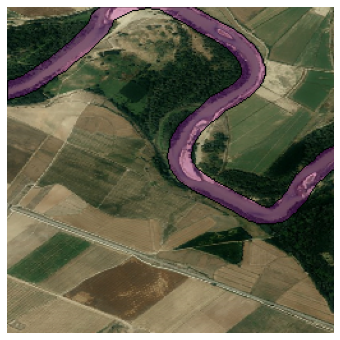
\includegraphics[width=0.40\columnwidth]{Imagenes/caso-practico/ebro1.png}}
    \subfigure{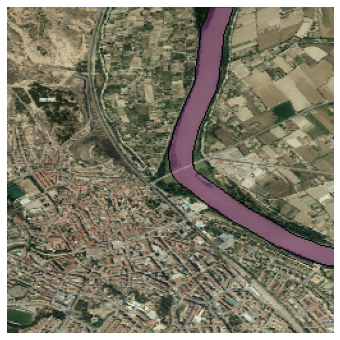
\includegraphics[width=0.40\columnwidth]{Imagenes/caso-practico/ebro2.png}}
    \caption{Selección del río Ebro en distintos tramos} \label{fig:ebro} 
\end{figure} 

El siguiente código genera como resultado las imágenes mostradas en la figura \ref{fig:ebro},
en las que se muestra el cauce del río Ebro seleccionado (capa elaborada en la primera parte) sobre el mapa base con ortofoto.
\newpage
\begin{tcolorbox}[breakable, size=fbox, boxrule=1pt, pad at break*=1mm,colback=cellbackground, colframe=cellborder, fontupper=\footnotesize]
    \prompt{In}{incolor}{177}{\boxspacing}
    \begin{Verbatim}[commandchars=\\\{\}]
    \PY{n}{img\PYZus{}grow} \PY{o}{=} \PY{l+m+mf}{0.01}
    \PY{c+c1}{\PYZsh{} 2.1 Seleccionar aleatoriamente dos puntos de la capa del río Ebro}
    \PY{k}{for} \PY{n}{i}\PY{p}{,} \PY{n}{point} \PY{o+ow}{in} \PY{n+nb}{enumerate}\PY{p}{(}\PY{n}{random}\PY{o}{.}\PY{n}{choices}\PY{p}{(}\PY{n}{ebro\PYZus{}points}\PY{p}{,} \PY{n}{k}\PY{o}{=}\PY{l+m+mi}{2}\PY{p}{)}\PY{p}{)}\PY{p}{:}
        \PY{k}{try}\PY{p}{:}
            \PY{c+c1}{\PYZsh{} 2.2 Generar bounding box a partir de un punto del río ebro }
            \PY{n}{img\PYZus{}bbox\PYZus{}coord} \PY{o}{=} \PY{n}{get\PYZus{}bbox\PYZus{}coord}\PY{p}{(}\PY{n}{point}\PY{p}{,} \PY{n}{img\PYZus{}grow}\PY{p}{)}
    
            \PY{c+c1}{\PYZsh{} 2.3 Descarga de la imágen del servicio WMS de IDENA}
            \PY{n}{parameters}\PY{p}{[}\PY{l+s+s1}{\PYZsq{}}\PY{l+s+s1}{BBOX}\PY{l+s+s1}{\PYZsq{}}\PY{p}{]} \PY{o}{=} \PY{l+s+s2}{\PYZdq{}}\PY{l+s+s2}{,}\PY{l+s+s2}{\PYZdq{}}\PY{o}{.}\PY{n}{join}\PY{p}{(}\PY{n+nb}{str}\PY{p}{(}\PY{n}{coord}\PY{p}{)} \PY{k}{for} \PY{n}{coord} \PY{o+ow}{in} \PY{n}{img\PYZus{}bbox\PYZus{}coord}\PY{p}{)}
            \PY{n}{response} \PY{o}{=} \PY{n}{requests}\PY{o}{.}\PY{n}{get}\PY{p}{(}\PY{n}{url}\PY{p}{,} \PY{n}{params}\PY{o}{=}\PY{n}{parameters}\PY{p}{,} \PY{n}{stream}\PY{o}{=}\PY{k+kc}{True}\PY{p}{)}
            \PY{n}{img} \PY{o}{=} \PY{n}{Image}\PY{o}{.}\PY{n}{open}\PY{p}{(}\PY{n}{io}\PY{o}{.}\PY{n}{BytesIO}\PY{p}{(}\PY{n}{response}\PY{o}{.}\PY{n}{content}\PY{p}{)}\PY{p}{)}
    
            \PY{c+c1}{\PYZsh{} 2.4 Generar intersección entre el bbox y la capa del río Ebro}
            \PY{n}{lon\PYZus{}min}\PY{p}{,} \PY{n}{lat\PYZus{}min}\PY{p}{,} \PY{n}{lon\PYZus{}max}\PY{p}{,} \PY{n}{lat\PYZus{}max} \PY{o}{=} \PY{n}{img\PYZus{}bbox\PYZus{}coord}
            \PY{n}{img\PYZus{}bbox} \PY{o}{=} \PY{n}{gpd}\PY{o}{.}\PY{n}{GeoSeries}\PY{p}{(}\PY{p}{[}\PY{n}{Polygon}\PY{p}{(}\PY{p}{[}\PY{p}{(}\PY{n}{lon\PYZus{}min}\PY{p}{,} \PY{n}{lat\PYZus{}max}\PY{p}{)}\PY{p}{,} \PY{p}{(}\PY{n}{lon\PYZus{}max}\PY{p}{,} \PY{n}{lat\PYZus{}max}\PY{p}{)}\PY{p}{,} \PY{p}{(}\PY{n}{lon\PYZus{}max}\PY{p}{,} \PY{n}{lat\PYZus{}min}\PY{p}{)}\PY{p}{,} \PY{p}{(}\PY{n}{lon\PYZus{}min}\PY{p}{,} \PY{n}{lat\PYZus{}min}\PY{p}{)}\PY{p}{]}\PY{p}{)}\PY{p}{]}\PY{p}{)}
            \PY{n}{img\PYZus{}bbox\PYZus{}gdf} \PY{o}{=} \PY{n}{gpd}\PY{o}{.}\PY{n}{GeoDataFrame}\PY{p}{(}\PY{p}{\PYZob{}}\PY{l+s+s1}{\PYZsq{}}\PY{l+s+s1}{geometry}\PY{l+s+s1}{\PYZsq{}}\PY{p}{:} \PY{n}{img\PYZus{}bbox}\PY{p}{\PYZcb{}}\PY{p}{)}
            \PY{n}{img\PYZus{}bbox\PYZus{}gdf} \PY{o}{=} \PY{n}{img\PYZus{}bbox\PYZus{}gdf}\PY{o}{.}\PY{n}{set\PYZus{}crs}\PY{p}{(}\PY{n}{epsg} \PY{o}{=} \PY{l+m+mi}{4326}\PY{p}{)}
            \PY{n}{intersectionGDF} \PY{o}{=} \PY{n}{rioEbroGDF}\PY{o}{.}\PY{n}{overlay}\PY{p}{(}\PY{n}{img\PYZus{}bbox\PYZus{}gdf}\PY{p}{,} \PY{n}{how}\PY{o}{=}\PY{l+s+s1}{\PYZsq{}}\PY{l+s+s1}{intersection}\PY{l+s+s1}{\PYZsq{}}\PY{p}{)} 
            
            \PY{c+c1}{\PYZsh{} 2.5 Añadir la intersección obtenida en el mapa base}
            \PY{n}{draw} \PY{o}{=} \PY{n}{ImageDraw}\PY{o}{.}\PY{n}{Draw}\PY{p}{(}\PY{n}{img}\PY{p}{,} \PY{l+s+s1}{\PYZsq{}}\PY{l+s+s1}{RGBA}\PY{l+s+s1}{\PYZsq{}}\PY{p}{)}
            \PY{n}{poly\PYZus{}coords} \PY{o}{=} \PY{n}{intersectionGDF}\PY{o}{.}\PY{n}{geometry}\PY{p}{[}\PY{l+m+mi}{0}\PY{p}{]}\PY{o}{.}\PY{n}{exterior}\PY{o}{.}\PY{n}{coords}\PY{p}{[}\PY{p}{:}\PY{o}{\PYZhy{}}\PY{l+m+mi}{1}\PY{p}{]}
            \PY{n}{river\PYZus{}coord} \PY{o}{=} \PY{p}{[}\PY{n}{convert\PYZus{}latlon\PYZus{}pxpy}\PY{p}{(}\PY{n}{poly\PYZus{}coord}\PY{p}{[}\PY{l+m+mi}{1}\PY{p}{]}\PY{p}{,} \PY{n}{poly\PYZus{}coord}\PY{p}{[}\PY{l+m+mi}{0}\PY{p}{]}\PY{p}{,} \PY{n}{img\PYZus{}bbox\PYZus{}coord}\PY{p}{,} \PY{n}{img}\PY{p}{)} \PY{k}{for} \PY{n}{poly\PYZus{}coord} \PY{o+ow}{in} \PY{n}{poly\PYZus{}coords}\PY{p}{]}
            \PY{n}{draw}\PY{o}{.}\PY{n}{polygon}\PY{p}{(}\PY{n}{river\PYZus{}coord}\PY{p}{,} \PY{n}{fill}\PY{o}{=}\PY{p}{(}\PY{l+m+mi}{255}\PY{p}{,} \PY{l+m+mi}{0}\PY{p}{,} \PY{l+m+mi}{255}\PY{p}{,} \PY{l+m+mi}{50}\PY{p}{)}\PY{p}{,} \PY{n}{outline}\PY{o}{=}\PY{p}{(}\PY{l+m+mi}{0}\PY{p}{,}\PY{l+m+mi}{0}\PY{p}{,}\PY{l+m+mi}{0}\PY{p}{,}\PY{l+m+mi}{255}\PY{p}{)}\PY{p}{)}
    
            \PY{c+c1}{\PYZsh{} 2.6 Mostrar los resultados}
            \PY{n}{plt}\PY{o}{.}\PY{n}{figure}\PY{p}{(}\PY{n}{figsize}\PY{o}{=}\PY{p}{(}\PY{l+m+mi}{8}\PY{p}{,} \PY{l+m+mi}{6}\PY{p}{)}\PY{p}{)}
            \PY{n}{plt}\PY{o}{.}\PY{n}{imshow}\PY{p}{(}\PY{n}{img}\PY{p}{)}
            \PY{n}{plt}\PY{o}{.}\PY{n}{axis}\PY{p}{(}\PY{l+s+s1}{\PYZsq{}}\PY{l+s+s1}{off}\PY{l+s+s1}{\PYZsq{}}\PY{p}{)}
        \PY{k}{except} \PY{n+ne}{Exception} \PY{k}{as} \PY{n}{err}\PY{p}{:}
            \PY{n+nb}{print}\PY{p}{(}\PY{n}{err}\PY{p}{)}
            \PY{k}{continue}
    \end{Verbatim}
\end{tcolorbox}


